%%=====================================================================
%% METODOLOGIA
%%=====================================================================
\secaoudesc{Metodologia}

\begin{frame}{Arquitetura}
  \begin{columns}[c]
    \begin{column}{0.38\textwidth}
      \begin{itemize}
        \item \alert{SIBA}: aerodinâmica e bateria
        \item \alert{SAME}: tensões e correntes do motor
        \item Supervisório via TCP/UDP
      \end{itemize}
    \end{column}
    \begin{column}{0.62\textwidth}
      \centering
      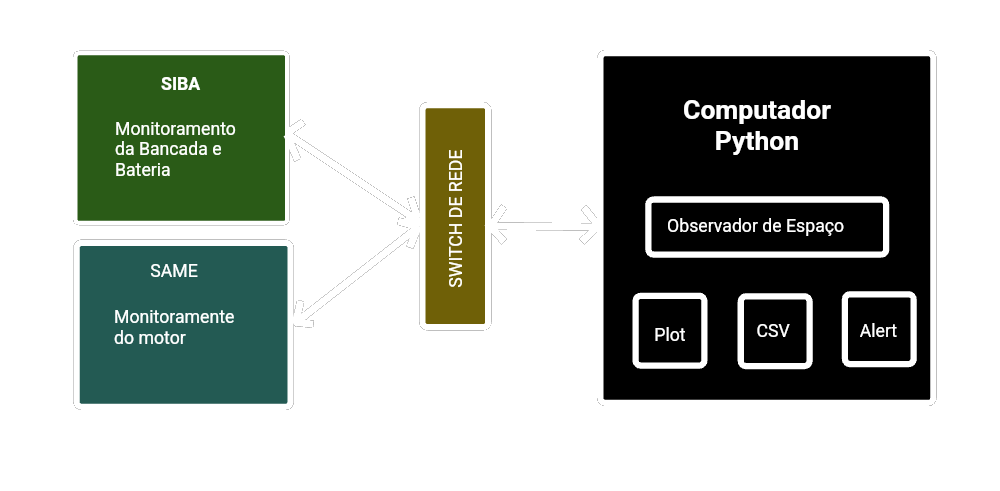
\includegraphics[width=\linewidth]{Metodologia/Arquitetura.png}
      \fonte[Autor; An (2026)]
    \end{column}
  \end{columns}
\end{frame}

\begin{frame}{Modelo do motor}
  \[
    \begin{bmatrix} v_\alpha \\ v_\beta \end{bmatrix}
    = R_s \begin{bmatrix} i_\alpha \\ i_\beta \end{bmatrix}
    + L_s \frac{\mathrm{d}}{\mathrm{d}t}
      \begin{bmatrix} i_\alpha \\ i_\beta \end{bmatrix}
    + \begin{bmatrix} e_\alpha \\ e_\beta \end{bmatrix}
  \]
  \[
    \hat{T}_e = \frac{3p}{4\,\hat{\omega}_e}
      \left(\hat{e}_\alpha i_\alpha + \hat{e}_\beta i_\beta\right)
  \]
  \fonte[Clarke (1943); Fitzgerald, Kingsley e Umans (2014); Krishnan (2017)]
\end{frame}

\begin{frame}{Observador por modos deslizantes}
  \begin{columns}[c]
    \begin{column}{0.36\textwidth}
      \begin{itemize}
        \item SMO estima a FEM
        \item PLL extrai ângulo e velocidade
        \item Reconstrução analítica da FEM
      \end{itemize}
    \end{column}
    \begin{column}{0.64\textwidth}
      \centering
      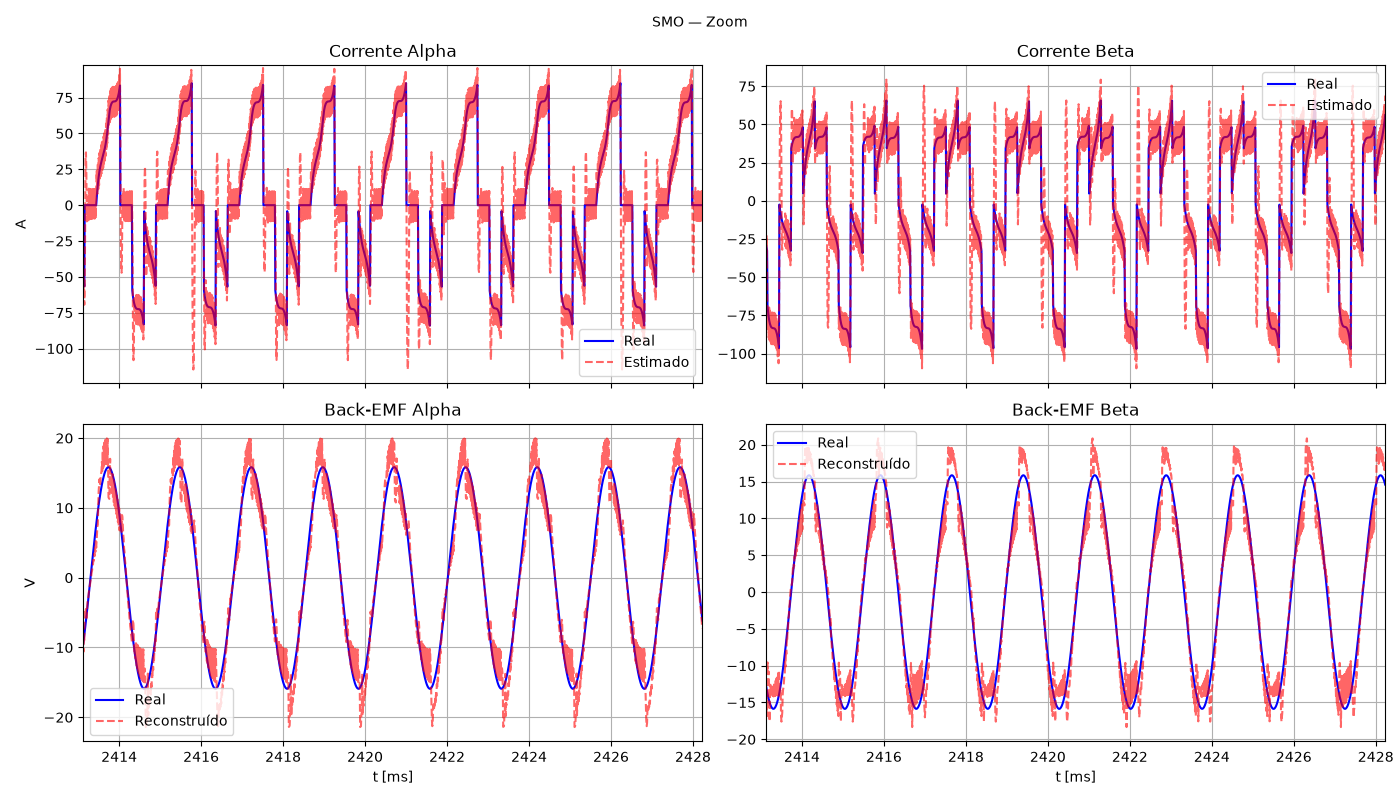
\includegraphics[width=\linewidth]{Desenvolvimento/reconstrucao_backemf.png}
      \fonte[Adaptado de Utkin (1992); Young, Utkin e Özgüner (1999); Abo Kaf et al.\ (2024)]
    \end{column}
  \end{columns}
\end{frame}

\begin{frame}{Ajuste automático dos ganhos}
  \begin{columns}[c]
    \begin{column}{0.36\textwidth}
      \begin{itemize}
        \item Evolução Diferencial
        \item Custo: torque + rotação
        \item Ganhos independentes do passo de amostragem
      \end{itemize}
    \end{column}
    \begin{column}{0.64\textwidth}
      \centering
      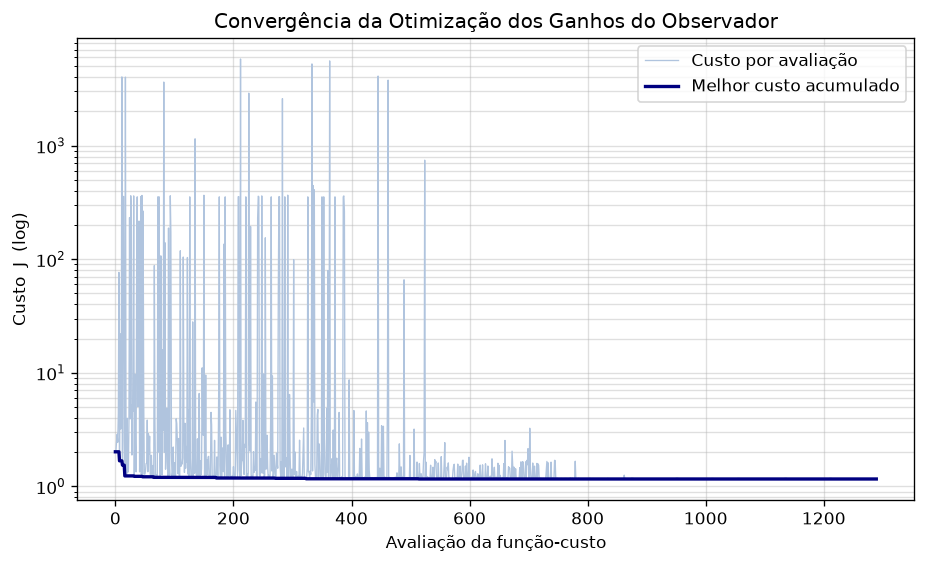
\includegraphics[width=\linewidth]{Desenvolvimento/Otim_convergencia.png}
      \fonte[Autor; Slotine e Li (1991)]
    \end{column}
  \end{columns}
\end{frame}

\begin{frame}{Hardware}
  \centering
  \begin{columns}[t]
    \begin{column}{0.33\textwidth}
      \centering
      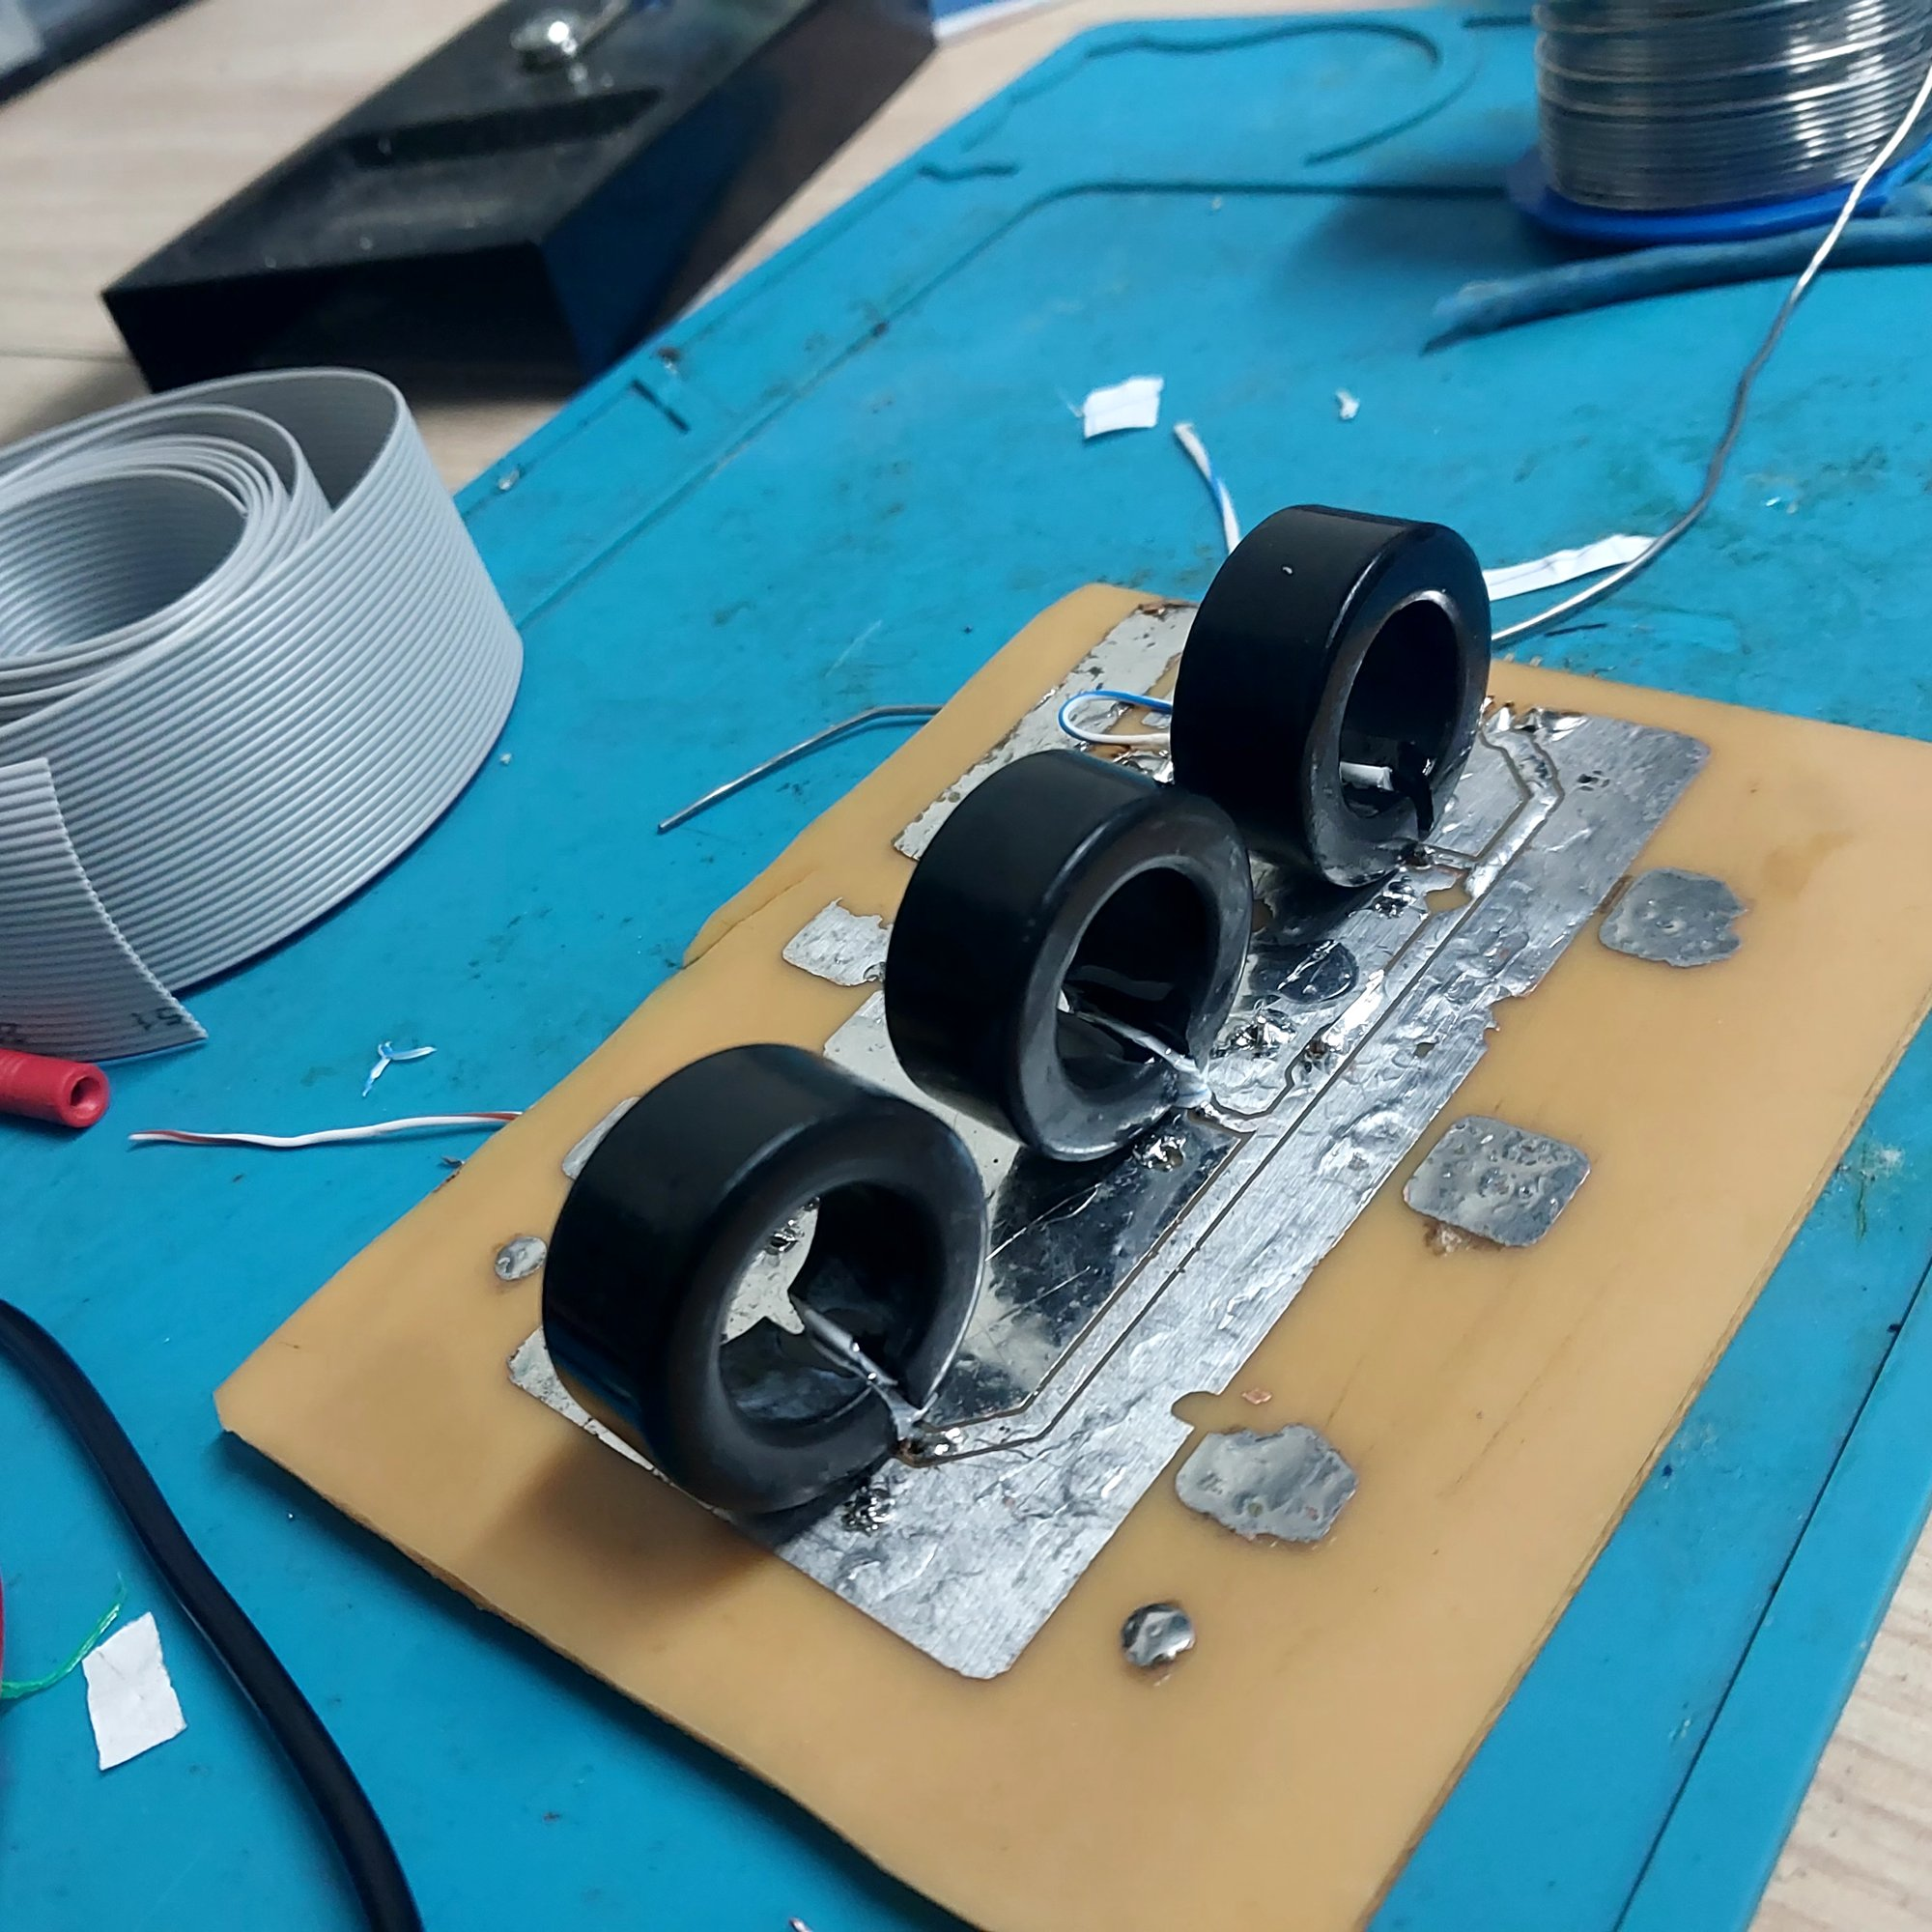
\includegraphics[height=0.5\textheight,width=0.95\linewidth,keepaspectratio]{Resultados/pcb_feita_aq1.jpg}\\[0.3em]
      {\small Placa AQ1}
    \end{column}
    \begin{column}{0.33\textwidth}
      \centering
      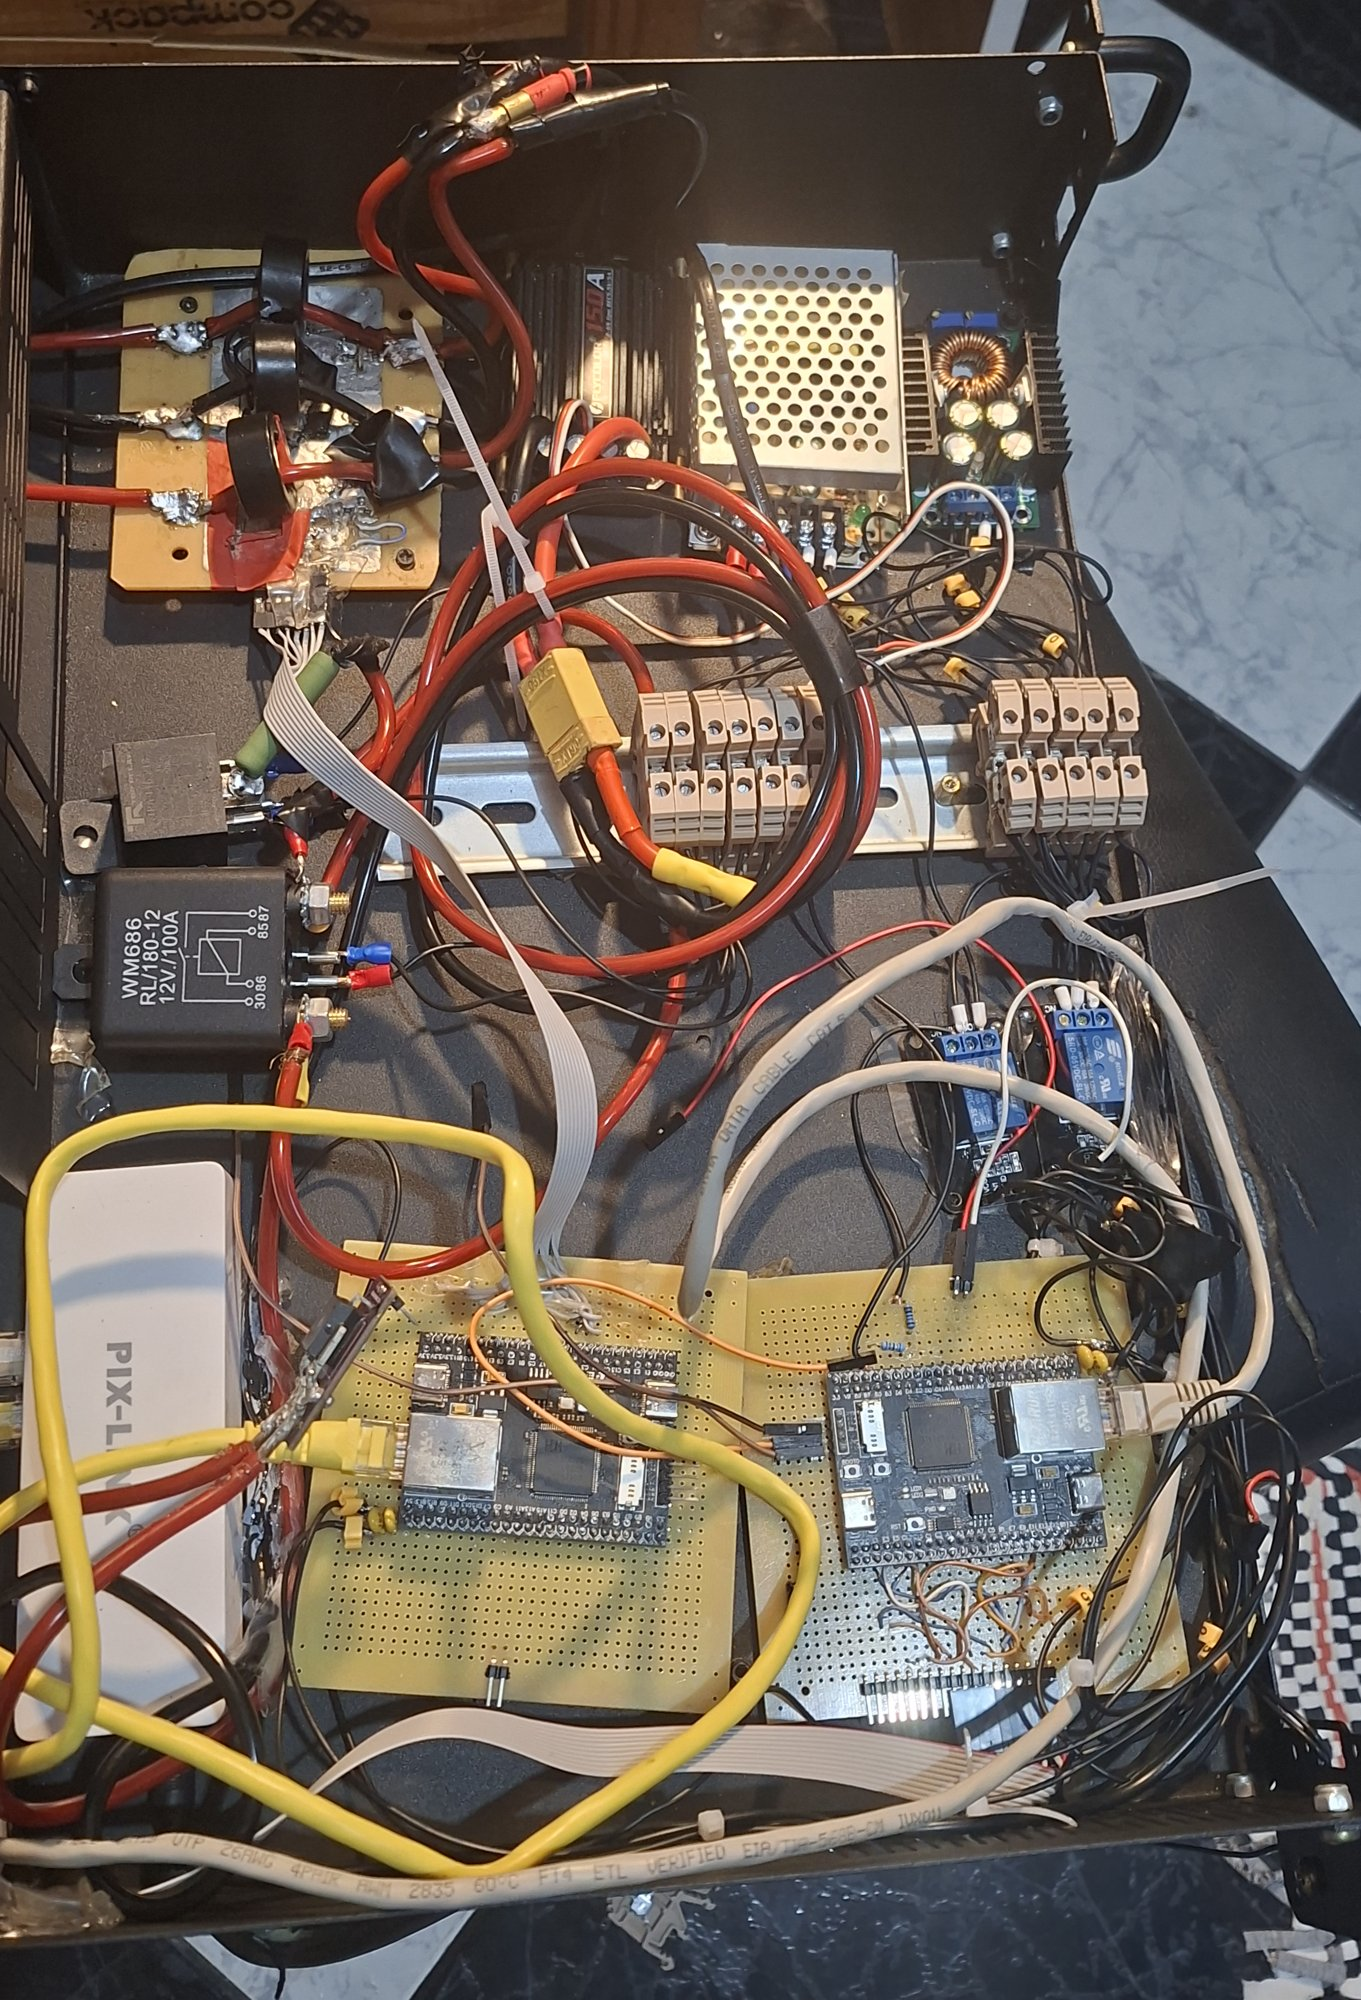
\includegraphics[height=0.5\textheight,width=0.95\linewidth,keepaspectratio]{Resultados/montagem_finalizada.jpg}\\[0.3em]
      {\small Fiação}
    \end{column}
    \begin{column}{0.33\textwidth}
      \centering
      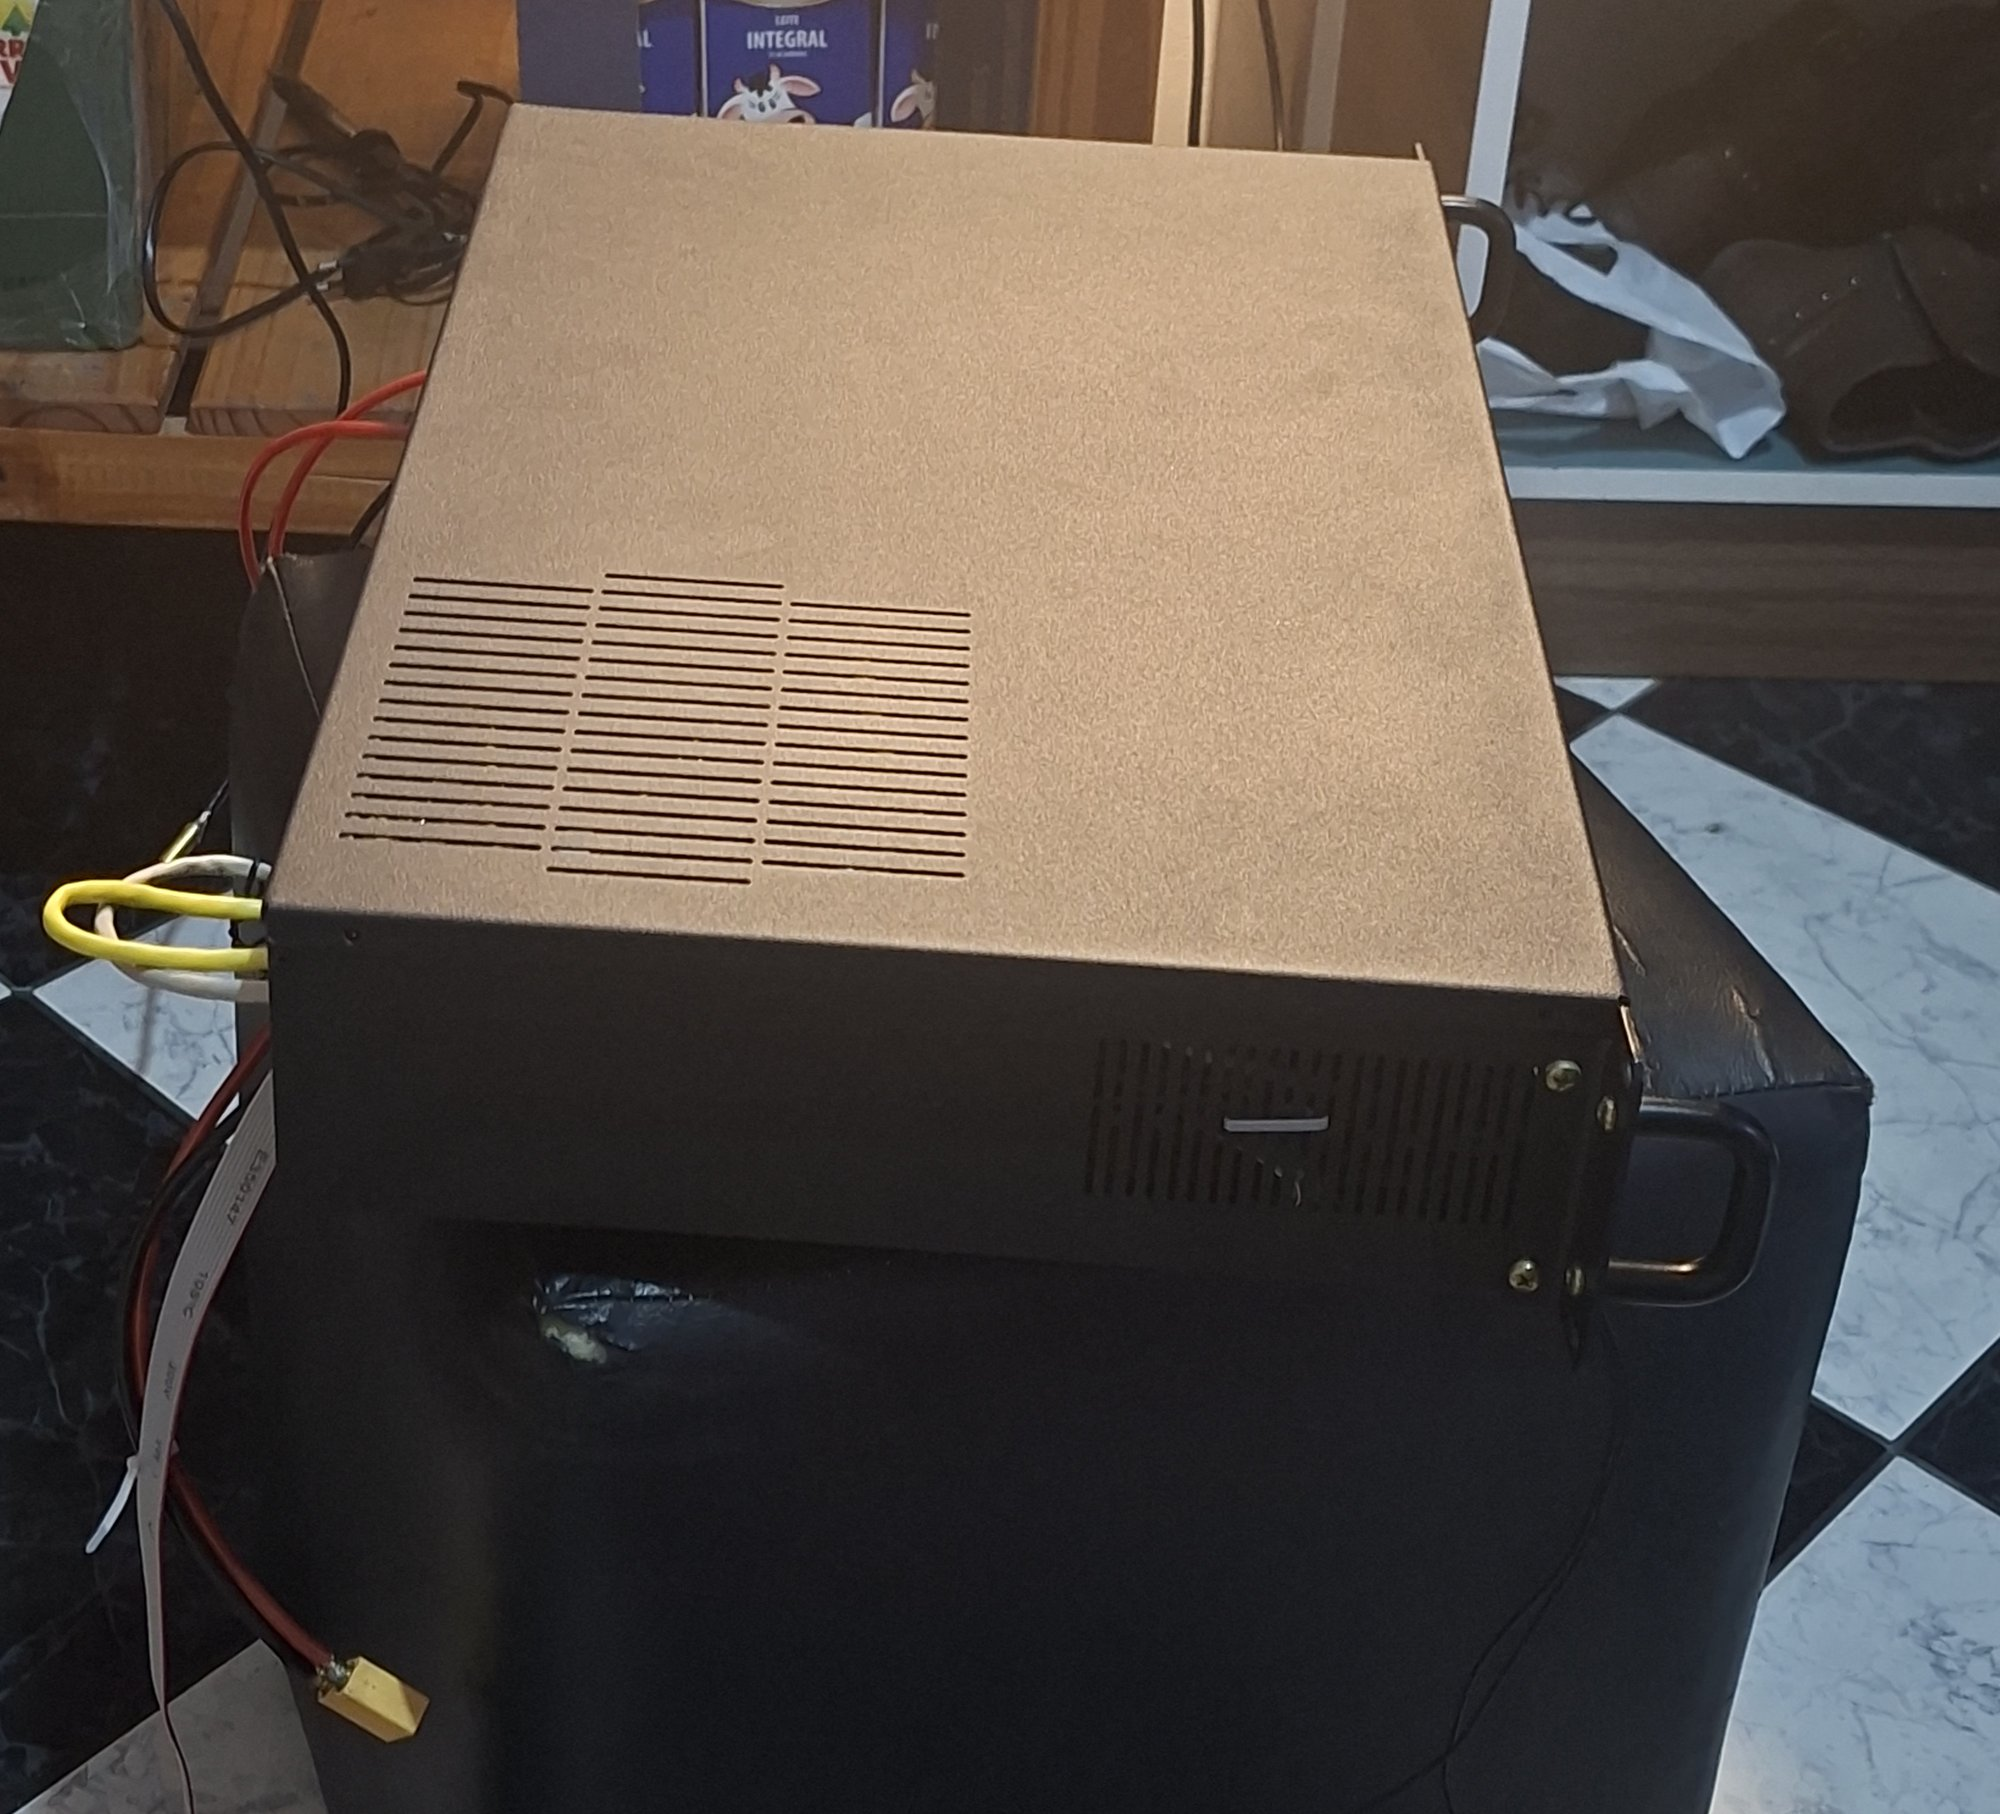
\includegraphics[height=0.5\textheight,width=0.95\linewidth,keepaspectratio]{Metodologia/gabinete.jpg}\\[0.3em]
      {\small Gabinete}
    \end{column}
  \end{columns}
  \vspace{0.6em}
  \fonte[Autor; Nanjing Qinheng Microelectronics (2026); Northrup (2018)]
\end{frame}

\begin{frame}{Firmware}
  \begin{columns}[c]
    \begin{column}{0.4\textwidth}
      \begin{itemize}
        \item Zephyr RTOS em CH32V307
        \item Fila de trabalho única
        \item Mesmo núcleo para SIBA e SAME
      \end{itemize}
    \end{column}
    \begin{column}{0.6\textwidth}
      \centering
      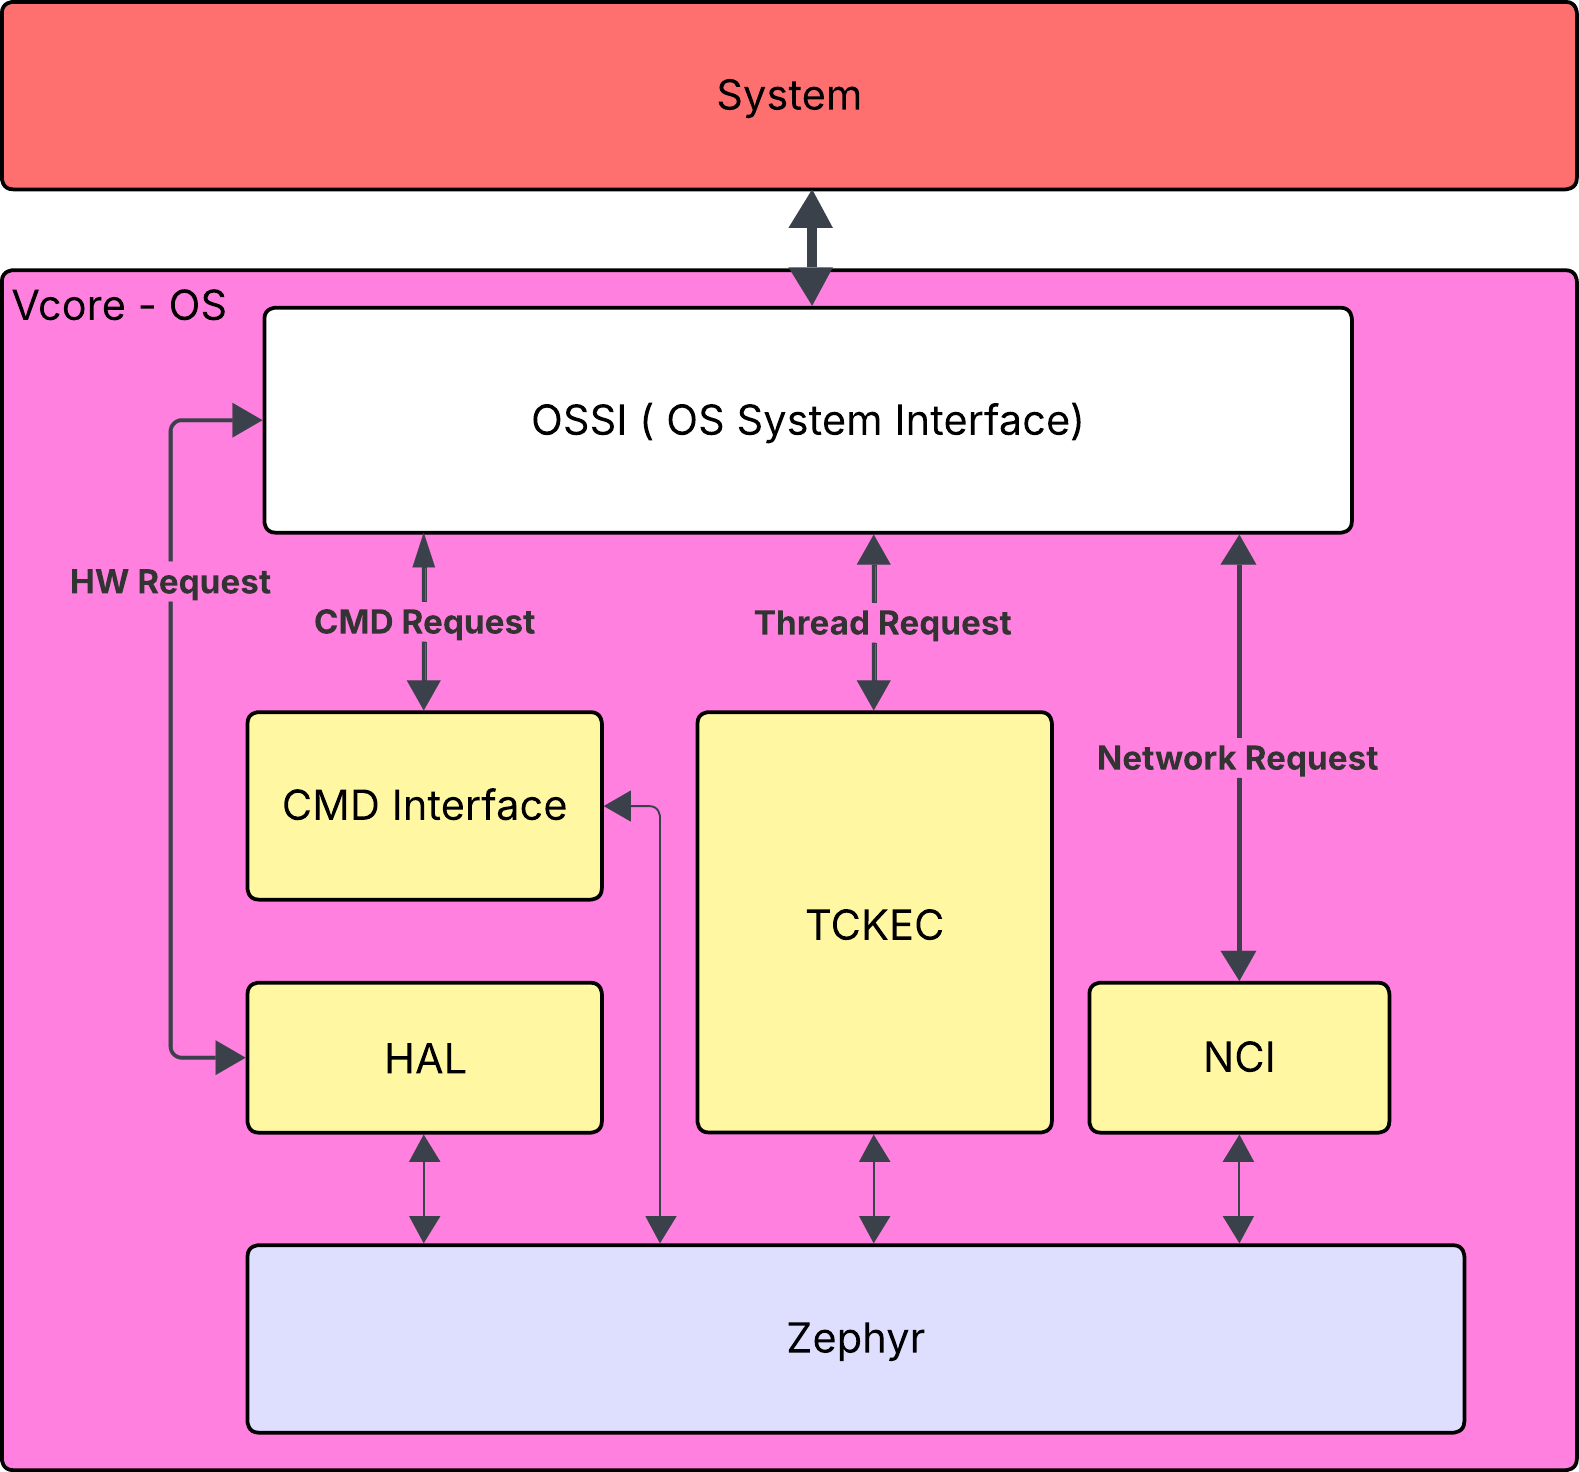
\includegraphics[height=0.72\textheight]{Metodologia/Vcore.png}
      \fonte[Adaptado de Zephyr Project (2026a; 2026b)]
    \end{column}
  \end{columns}
\end{frame}

\begin{frame}{Supervisório}
  \begin{columns}[c]
    \begin{column}{0.62\textwidth}
      \centering
      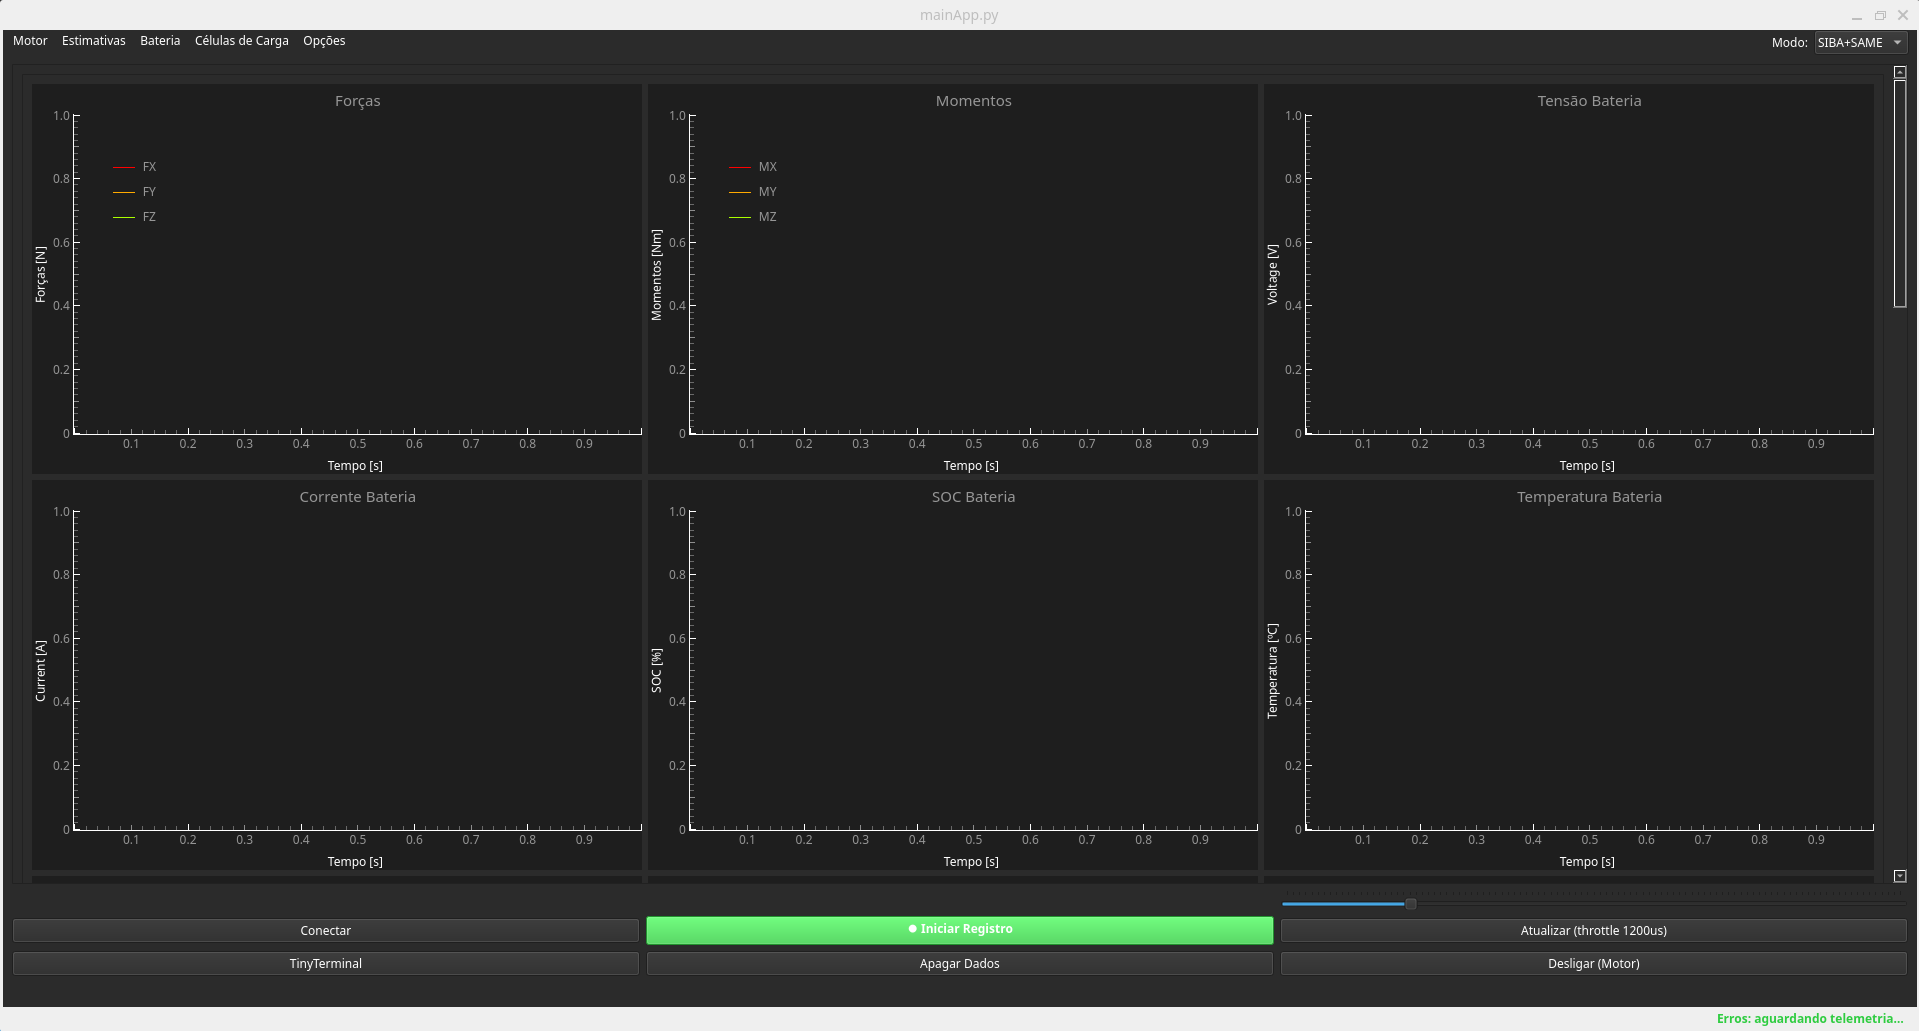
\includegraphics[width=\linewidth]{Metodologia/gui tela principal.png}
      \fonte
    \end{column}
    \begin{column}{0.38\textwidth}
      \centering
      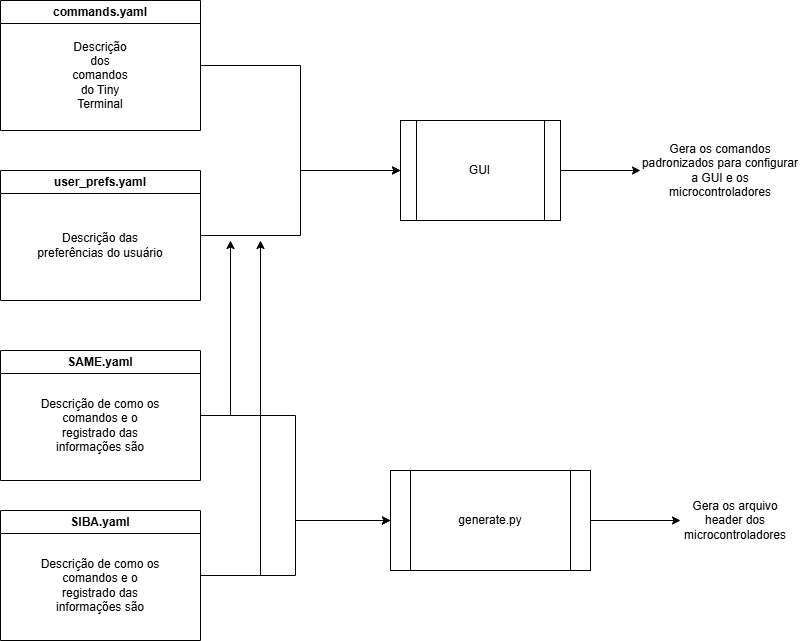
\includegraphics[width=0.85\linewidth]{Metodologia/YAML_uso.drawio.png}\\[0.3em]
      {\small YAML como fonte única para GUI e firmware}
    \end{column}
  \end{columns}
\end{frame}
